
\documentclass[11pt,a4paper]{article}

\usepackage[utf8]{inputenc} 
\usepackage[T1]{fontenc} 
\usepackage{lmodern}
\usepackage{tcolorbox}


\usepackage[german]{babel}


\setlength{\parindent}{0pt}
\setlength{\parskip}{1ex plus 0.5ex minus 0.5ex}

\usepackage{amsmath} 


\usepackage{graphicx} 

\usepackage[section]{placeins}
\usepackage{booktabs}


\usepackage{hyperref}
\hypersetup{
	colorlinks,
	citecolor=red,
	filecolor=black,
	linkcolor=black,
	urlcolor=black}
\graphicspath{}

\begin{document}
	
	{
		\centering 
		\large 
		Physiklabor für Anfänger*innen \\
		Ferienpraktikum im Sommersemester 2018 \\[4mm]
		\textbf{\LARGE 
			Versuch 75: Lichtmikroskop
		} \\[3mm]
		(durchgeführt am 02.10.2018 bei Daniel Bartle) \\
		Ye Joon Kim, Marouan Zouari\\
		\today \\[10mm]
	}
	\tableofcontents
\section{Einleitung}
Mit einer Lupe oder einem Mikroskop können kleine Objekte oder feine Einzelheiten stark vergrößert angesehen werden. Wie groß ein Objekt aussieht, hängt von dem Sehwinkel, $\epsilon =\arctan(B/b)$ ab (Siehe Abbildung 1). Eine Lupe lenkt das Licht so ab, sodass der Sehwinkel vergrößert wird. Dadurch wird ein vergrößerndes Bild in dem Auge geschafft. Die Vergrößerung ist definiert durch:
\begin{equation}
V = \frac{\varepsilon}{\varepsilon_0}
\end{equation}

Wobei $\varepsilon_0$ und $\varepsilon$ jeweils der Sehwinkel ohne und mit der Lupe sind. Für sehr kleine Winkel gilt $\varepsilon \approx \tan(\varepsilon)$, und dadurch lässt sich $V$ auch schreiben als:
\begin{equation}
V \approx \frac{\tan\varepsilon}{\tan\varepsilon_0} = \frac{G/f}{G/s_0} = \frac{s_0}{f}
\end{equation}

Ein Mikroskop funktioniert ähnlich, aber es kann viel stärkere Vergrößerungen schaffen. Die zwei wichtigsten Teile eines Mikroskops sind das Objektiv und das Okular. 

Das Licht von dem Objekt geht zuerst durch das Objektiv. Das Objektiv bricht das Licht so, sodass es am Brennpunkt des Okulars ein vergrößertes reelles Zwischenbild entsteht. Das Okular schickt, wie eine Lupe, das Licht in das Auge, wobei das Bild nochmals vergrößert wird (Siehe Abbildung 2). Mit nur diesen zwei Linsen können riesige Vergrößerungen geschafft werden. Die Vergrößerung eines Mikroskops kann so geschrieben werden:
\begin{equation}
V_\textrm{Mikroskop} \approx \frac{\tan\epsilon}{\tan\epsilon_0}= \frac{B/f_2}{G/s_0} = \frac{B}{G}\cdot\frac{s_0}{f} = \beta_\textrm{obj}\cdot V_\textrm{ok}
\end{equation}
Wobei $B$ und $G$ die jeweils Bild- und Gegenstandgröße bezüglich des Objektives, $\beta_\textrm{obj}$ der Abbildungsmaßstab des Objektives und $V_\textrm{ok}$ die Vergrößerung des Okulars sind. 


\begin{figure}
	\centering
	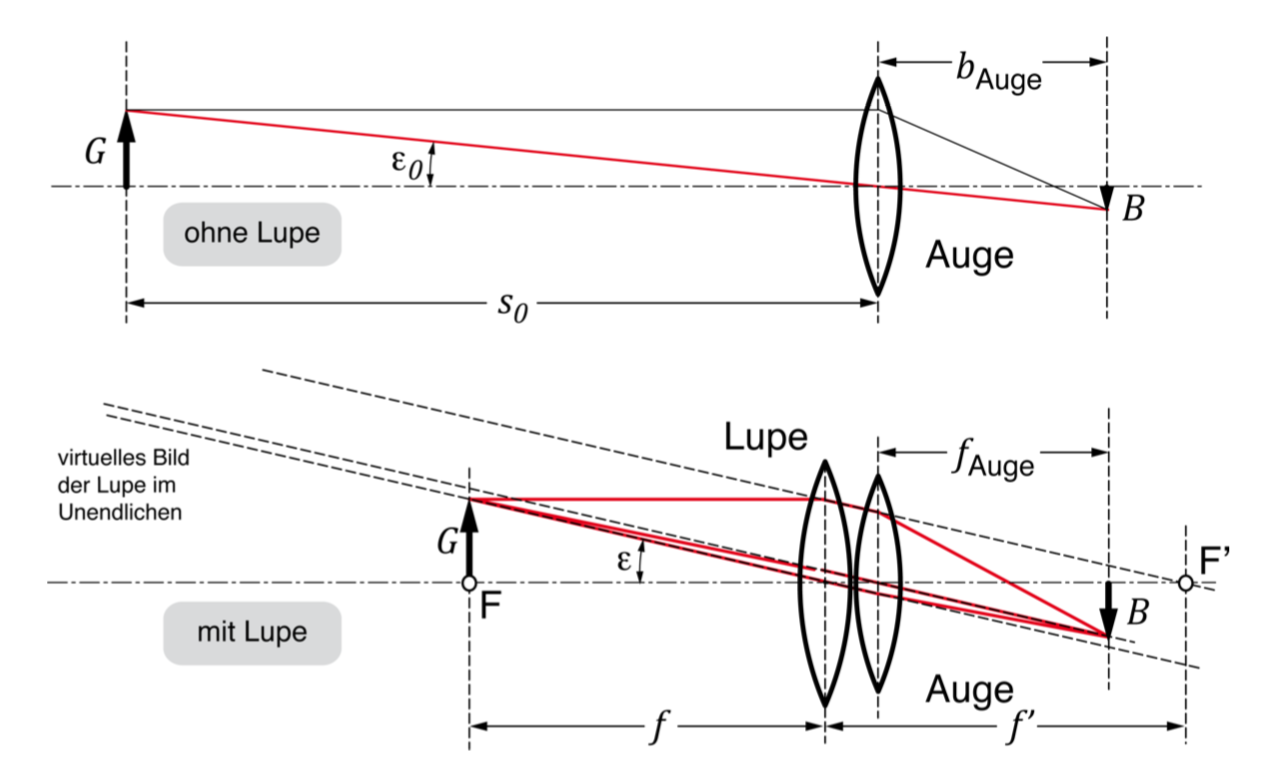
\includegraphics[width=\linewidth]{Abb1}
	\caption{Funktionsweise einer Lupe (,,Versuchsanleitungen'')}
\end{figure}

\begin{figure}
	\centering
	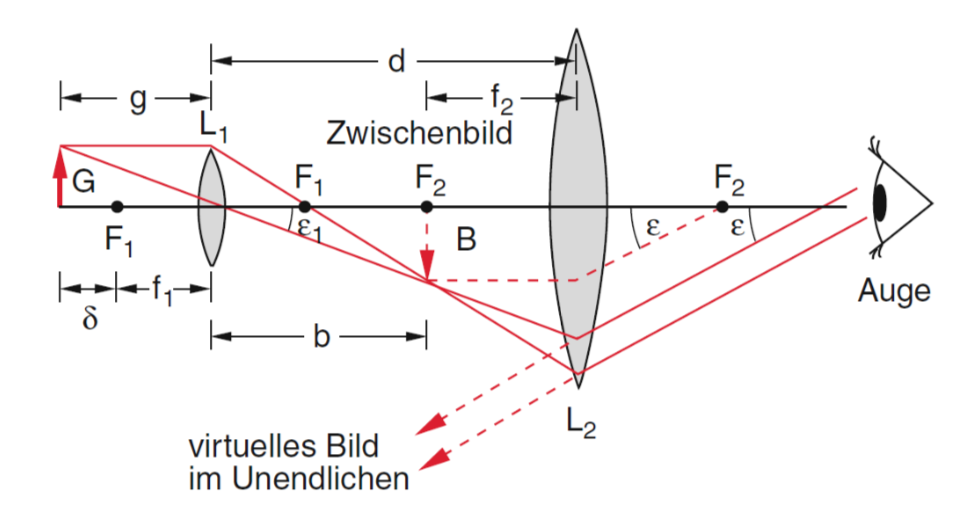
\includegraphics[width=\linewidth]{Abb2}
	\caption{Funktionsweise eines Lichtmikroskops(,,Versuchsanleitungen'')}
\end{figure}

Bei echten Mikroskope sind aber nicht nur die Vergrößerung aber auch die Beleuchtung wichtig. In diesem Versuch wird die Köhlersche Beleuchtung untersucht. Zu dem werden vier zusätzliche Bauteilen benötigt. 

Die Kollektorlinse bildet die Lichtquelle vergrößert auf die dahinten stehende Leuchtfeldblende ab. Der Hebel von der Leuchtfeldblende kann verstellt werden, um die Größe der Apertur zu ändern,  und dadurch kontrolliert die Blende wie groß die Abbildung auf dem Schirm ist. Daneben steht eine Aperturblende, die sich an dem Brennpunkt der dahinten stehenden Kondensorlinse befindet. Ähnlich wie die Leuchtfeldblende kann die Größe des Lochs an der Blende justiert werden, aber da die Blende sich am Brennpunkt der Kondensorlinse befindet, wird die Größe der Abbildung nicht beeinflusst, sondern nur ihre Helligkeit. Die Kondensorlinse bildet dann das Licht auf das Objektebene (Siehe Abbildung 3).

\begin{figure}
	\centering
	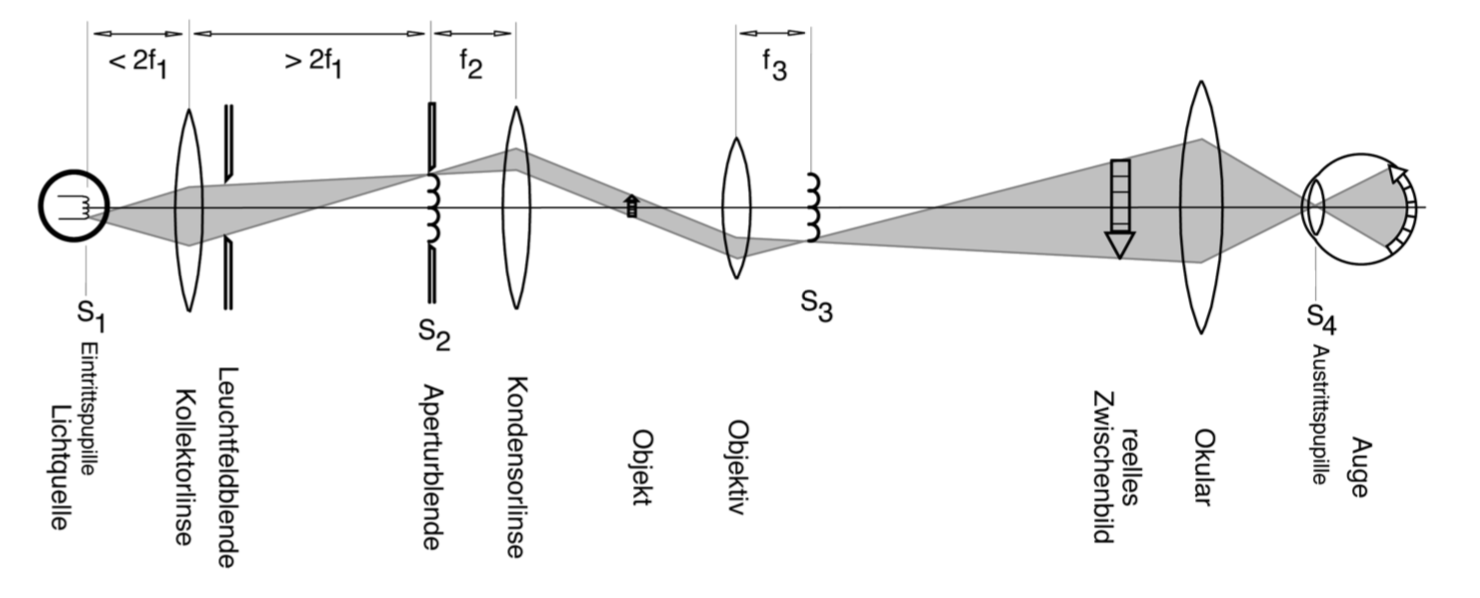
\includegraphics[width=\linewidth]{Abb3}
	\caption{Köhlersche Beleuchtung}
\end{figure}

\section{Aufbau}
Zum Versuch wurden die in dem obigen Abschnitt erwähnten optische Apparate, eine optische Bank, ein transparenter und opaker Schirm mit ein Stück Millimeterpapier, eine beleuchtete Referenzskala und zwei Objekte (Drahtgitter und Objektmikrometer) benutzt. 

\section{Durchführung}
Es wurden zuerst auf der optischen Bank der Schirm und Objektivelinse fixiert. Die Linse und Schirm wurden so verschoben, sodass es eine relativ scharfe vergrößerte Abbildung auf dem Schirm erzeugt wurde. Die Lichtquelle wurde justiert, sodass die Abbildung zentriert war.  

Für den ersten Versuchsteil wurde ein Drahtgitter vor dem Objektiv bei Position 250mm eingesetzt. Das Objektiv wurde dann verschoben, damit eine scharfe Abbildung des Gitters entstanden war. Dann wurde eine Kollektorlinse direkt vor der Lichtquelle fixiert. Ihre Position wurde variiert und der Einfluss auf die Beleuchtung wurde beobachtet. Die Aperturblende wurde dann zwischen dem Objekt und der Kollektorlinse eingesetzt. Es wurde dann untersucht am welcher Stelle der ausgeleuchtete Bereich nicht geändert wurde, wenn die Aperturblende gedreht wurde. Eine Leuchtfeldblende wurde dann zwischen der Aperturblende und Kollektorlinse fixiert und es wurde untersucht ob die Position der Kollektorlinse einen Enfluss auf die Beleuchtung hat. 

Für den zweiten Teil wurden die Bauteile ein Bisschen justiert, um das Objekt optimal abbilden zu können. Die Kollektorlinse wurde am Position 11,5 cm, die Leuchtfeldblende am Position 12,7 cm, die Aperturblende am Position 19,2 cm, die Kondensatorlinse am Position 25,0 cm, das Objekt am Position 30,7 cm, das Objektiv am Position 35,8 cm und der Schirm am Position 119,0 cm fixiert. Für das Objekt wurde das Objektmikrometer benutzt. Die Größe einer abgebildeten Skala wurde dann mit der Millimeterpapier auf dem Schirm gemessen. Danach wurde die Abstände zwischen dem Objekt und Objektiv und dem Bild und Objektiv gemessen. 

Für den dritten Versuchsteil wurde das Okular 50 mm hinter dem Schirm fixiert und der Würfel direkt dahinter. Die Referenzskala wurde dann 120mm hinter dem Würfel eingesetzt. 


\section{Auswertung und Fehleranalyse}

\section{Diskussion der Ergebnisse}

\section{Literatur}

\section{Anhang}

\end{document}